\section{Search for Similar Smart Contracts}
\label{appendix:sim_code}

The difficulty in code similarity lies in structural features of high-level language and diversity in the forms of logical expression of smart contracts. At present, there are various schools of code similarity algorithm in the academic circles, which are generally described as follows: 

%代码相似度的主要难点在于智能合约高级语言的结构性特点和逻辑表达形式的多样性。目前学术界对代码相似度的算法大概有下面这些流派:

\begin{itemize}
	\item \textbf{Edit Distance between Character Strings} \\
	Both of the entered query code and candidate source code are deemed as texts. Edit distance between two character strings is used for measuring similarity between them. Edit Distance refers to the minimum number of editing operations required for converting one character string into the other character string. Permitted editing operations include replacement of one character with another character, i.e. insertion of a character and deletion of a character. Generally speaking, the shorter the edit distance, the higher the similarity between two character strings. This algorithm based on edit distance between character strings can be used not only for source code comparison but also in intermediate representation or even machine language.
	For the purpose of improving the robustness of the algorithm based on edit distance between character strings, a certain degree of conversion of the source code without any semantic change will be conducted, such as removal of blank character, removal of annotation, replacement of names of all local variables with ‘\$’, normalized expression of algebraic expression, etc. This algorithm is characterized by fast speed, conciseness and high efficiency. However, its adaptability to complex programs is relatively poor and doesn't take syntax and organizational structure of code into consideration. 
	%\item 字符串编辑距离 
	%把输入query代码和候选源代码都当做文本,利用字符串编辑距离来衡量字符串之间的相似度。编辑距离(Edit Distance)指的两个字符串之间,由一个转成另一个所需的最少编辑操作次数。许可的编辑操作包括将一个字符替换成另一个字符,插入一个字符,删除一个字符。一般来说,编辑距离越小,两个串的相似度越大。这种字符串编辑距离算法既可以用在源代码比较,也可以用在中间语言(intermediate representation),甚至可以用在机器语言中。

	%为了提高字符串编辑距离算法的健壮性,会对源代码做一些不改变语义的转换,例如:去除空白字符,去除注释,局部变量名统一用'\$'代替,代数表达式的归一化表达等。该算法运算速度快,简洁高效,但是对于复杂程序适应性较差,完全没有考虑到代码的语法和组织结构。

	\item \textbf{Token Sequence} \\
	Token sequence representation method refers to the conversion of the entered source code into a Token sequence through the analysis by a lexical analyzer. Similarity between two programs is similarity between two Token sequences, so the longest common substring or correlation matching algorithm (suffix tree matching algorithm) may be used to measure the degree of similarity between two programs, through which code segments with different syntaxes but similar functions can be detected. However, this method conceals organizational structure of programs when measuring the similarity between two programs.
	%Token序列表示法是将输入的源代码通过词汇分析器分析,将源代码转换成Token序列。两个程序的相似度就是Token序列的相似度,可以用最长公共子串,或者相关匹配算法(如后缀树匹配算法)度量程序间的相似程度,这样做可以检测出具有不同句法但却有相似功能的代码段,但该方法在程序相似度度量时隐藏了程序的组织结构。

	\item \textbf{Abstract Syntax Tree (AST)} \\
	AST is an intermediate expression form after syntactic analysis on a source code is conducted, based on which the similarity between two programs can be measured through comparison between one subtree and another subtree. For measurement of the similarity between two trees, the tree edit distance algorithm \cite{zhang1989simple} may be used. The accurate tree edit distance algorithm is relatively complex and Literature \cite{guha2002approximate} provides an approximate fast algorithm. According to Literature \cite{chilowicz2009syntax}, syntax tree should be subject to Hash fingerprint in order to enable the syntax tree comparison algorithm to conduct high-efficiency searching on massive datasets. 
	
	%抽象语法树(AST)是对源代码用语法分析后形成的中间表达形式,通过比较子树与其他子树之间的相似程度对程序的相似度进行度量。比较两棵树之间的相似度可以用树的编辑距离算法~\cite{zhang1989simple},精确的树编辑距离算法复杂度较大,文献~\cite{guha2002approximate}提供了一种近似的快速算法,文献~\cite{chilowicz2009syntax}提出对语法树做哈希指纹,使得语法树比较算法可以在海量数据集上进行高效检索。

	\item \textbf{Program Dependency Graph (PDG)} \\
	PDG \cite{ferrante1987program} can represent internal data and control dependency relationship of a program and analyze program code at the semantic level. Similar code protocol becomes search of isomorphic subgraphs, which is the NP-complete problem and requires a very complex algorithm, so only some approximate algorithms are available currently.

	%程序依赖图PDG~\cite{ferrante1987program}可以表示程序内部数据以及控制依赖关系,能够在语义级别上对程序代码进行分析。相似代码规约成为寻找同构子图,这是NP完全问题,算法复杂度很高,目前只能用一些近似算法。

\end{itemize}

We believe that the abovementioned algorithms describe similarity between codes in text, structure and syntax at different dimensions. Source Forager [27] provides a great engineering thought: Indexes of similarity at various dimensions are depicted as different features, each of which represents code similarity measurement from a specific aspect. Finally, vector similarity is used to conduct overall similarity measurement. This method integrates the advantages of the abovementioned algorithms. This thought is also used by Nebulas for reference in realizing search of similarity among smart contracts. We deem function as the fundamental unit of code search among smart contracts.

%我们认为上述各种算法都在不同维度描述了代码的文本、结构、语法上的相似度。Source Forager~\cite{kashyap2017source}提供了一个很好的工程思路,把各种不同维度的相似度指标刻画为不同的特征,每个特征都表征了代码某种方面的相似度衡量,最后用向量的相似度来做总体的相似度衡量,综合了以上各种算法的优点。星云链也借鉴这种思路,实现智能合约的相似搜索。我们把函数作为智能合约代码搜索的基本单位。

Table \ref{table:search-similarity} defines the candidate code similarity features. Next, we are going to describe definition of each feature and the function for calculating their similarity:

%表\ref{table:search-similarity}定义了候选的代码相似度特征,我们接下来进一步描述每个特征的定义和它们的相似度计算函数:


\begin{table}[h]
\centering
\begin{threeparttable}[b]
\caption{Code Similarity Feature Family Table}
\label{table:search-similarity}
\begin{tabular}{ccc} \toprule
    {Feature-Class} & {Brief Description} \\ \midrule
Type–Operation Coupling & types used and operations performed on the types \\
Skeleton Tree & structure of loops and conditionals \\
Decorated Skeleton Tree & structure of loops, conditionals, and operations \\
3 Graph CFG BFS & CFG subgraphs of size 3, BFS used for generating subgraphs \\
4 Graph CFG BFS & CFG subgraphs of size 4, BFS used for generating subgraphs \\
3 Graph CFG DFS & CFG subgraphs of size 3, DFS used for generating subgraphs \\
4 Graph CFG DFS & CFG subgraphs of size 4, DFS used for generating subgraphs \\
Library Calls & calls made to libraries \\
Type Signature & input types and the return type \\
Local Types & types of local variables \\
Numeric Literals & numeric data constants used \\
String Literals & string data constants used \\
\bottomrule                                                   
\end{tabular}
\end{threeparttable}
\end{table}

\begin{itemize}
	\item \textbf{Type–Operation Coupling} \\
	This feature is a two-tuple set. Two tuples contain type of variable and operator of type of variable, namely the (type, operation) pair. Generally, primitive data type should be paired with arithmetic operator, logical operator and relational operator, such as ($int, \geq$); custom data type (such as struct) should be paired with member function, such as (Bar, .foo), indicating that field ``foo" of data type ``Bar" is accessed. Based on this method, all operations on variables in the code body of a function can be changed into two-tuples. After repetition removal, A two-tuple sequence is used to reflect the Type–Operation Coupling feature of this code segment. We believe that codes with similar functions should have similar variable operation sets. However, we are not concerned with the order of the two tuples, so this feature loses the logical structure information of code and thus can only represent feature of code partially.
	
	%该特征是一个二元组集合,二元组包含变量类型,以及变量类型的算符,即(type, operation)对。原生数据类型一般和算术运算符、逻辑运算符以及关系运算符配对,例如($int, \geq$);自定义类型(例如struct)一般和成员函数配对,例如(Bar, .foo)表示数据类型Bar的字段foo被访问。按照这种方法,把一个函数的代码体内部所有变量操作都变成二元组,并且去重以后,就用一个二元组序列体现了这段代码的Type–Operation Coupling特征。我们认为相似功能的代码,也应该具有相似的变量操作集合。但是我们并不关心二元组的先后顺序,所以该特征丢失了代码的逻辑结构信息,只能部分代表代码的特征。
	
	Similarity among Type–Operation Coupling features can be defined by Jacobian similarity, namely that if two sets $S_1$ and $S_2$ are given, Jacobian similarity can be defined with the following formula:
	
	%Type–Operation Coupling特征之间的相似度可以由雅克比相似度定义,即如果给定两个集合$S_{1}$和$S_{2}$,雅克比相似度由如下公式定义:
	
	\begin{equation}
	sim_{Jacc(S_{1}, S_{2})}=\frac{\mid S_{1}\bigcap S_{2}\mid}{\mid S_{1}\bigcup S_{2}\mid}
	\end{equation}
	
	\item \textbf{Skeleton Tree} \\
	Code-based abstract syntax tree. However, only loop (for, while, do...while) and conditional statement (if...else) are reserved, and all the other nodes are removed from the tree. We believe that codes with similar functions should be similar in structure of loop and conditional statement.
	
	%基于代码的抽象语法树,但是只保留了循环(for, while, do...while)和条件语句(if...else),其余节点从树中全部移除。我们认为相似功能的代码,应该具有相似的循环和条件语句结构。
	
	Similarity calculation for skeleton tree is based on edit distance between two trees. $d_{r}$ is defined as the estimated edit distance between two trees and is only determined by size of tree, namely that:
	%Skeleton Tree的相似度计算基于树的编辑距离。定义$d_{r}$为两棵树的预估编辑距离,此距离仅仅由树的大小决定,即:
	
	\begin{equation}
	d_{r}(T_{1}, T{2})=\frac{\mid size(T_{1})-size(T_{2})\mid}{max(size(T_{1}), size(T_{2}))}
	\end{equation}
	
	$D_T$ is assumed as the threshold value of edit distance and set as 0.5. We can further acquire the formula for calculation of approximate edit distance between two trees:
	%假设$D_{T}$是编辑距离的阈值,设定为0.5。我们进一步得到两棵树的近似编辑距离公式:
	
	\begin{equation}
	d_{t}(T_{1}, T{2})=\begin{cases}d_{r}(T_{1}, T{2}) & if~d_{r}(T_{1}, T{2})\geq D_{T}\\\frac{max\left(\begin{array}{c}ed(pre(T_{1}),~pre(T_{2})),\\ ed(post(T_{1}),~post(T_{2}))\end{array}\right)}{max(size(T_{1}), size(T_{2}))} & otherwise\end{cases}
	\end{equation}
	
	pre(T) represents preorder traversal sequence of tree; post(T) represents postorder traversal sequence of tree; $ed(S_{1}, S_{2})$ represents edit distance between $S_{1}$ and $S_{2}$. Similarity between two skeleton trees can be calculated with the following formula:
	
	%pre(T)代表树的先序遍历序列,post(T)代表树的后序遍历序列,$ed(S_{1}, S_{2})$代表序列$S_{1}$和$S_{2}$的编辑距离。Skeleton Tree的相似度可以由以下公式计算:
	
	\begin{equation}
	sim_{Tree}(T_{1}, T{2})=1-d_{t}(T_{1}, T{2})
	\end{equation}
	
	\item \textbf{Decorated Skeleton Tree} \\
	Decorated Skeleton Tree is similar to Skeleton Tree. In addition to loop and branch node, most operators (such as +, -, <) are reserved. However, assignment operators are removed because most of these operators are noises.
	
	%和Skeleton Tree相似,除了循环和分支节点以外,还保留了大部分运算符(例如+, -, <)。但是赋值运算符去除了,因为这些大都是噪音。
	
	\item \textbf{K-Subgraphs of CFG} \\
	Realized based on k-subgraph of CFG of a function. k-subgraph should be defined with the following method: A CFG and a specific node should be given, based on which we should conduct breadth-first search (BFS) or depth-first search (DFS) until number of traversed nodes reaches k, when the formed subgraph should be k-subgraph. If number of nodes fails to reach k after finish of traversal, such subgraph should be discarded. Through traversal of each node of CFG, we can acquire all k-subgraphs. For each k-subgraph, $k^2$ bit integer is used to express it. Refer to Figure \ref{fig:graph-ex}. All k-subgraphs form one integer set.
	%基于函数的CFG图的k-子图实现。k-子图按如下方法定义:给定CFG图和某节点,我们做广度优先遍历(BFS)或者深度优先遍历(DFS),直至遍历节点数为k,形成的子图为k-子图。如果遍历结束后,节点数不足k,丢弃该子图。遍历CFG图的每个节点,我们可以得到所有的k-子图。对于每个k-子图,我们用$k^{2}$位整数表示,参考图\ref{fig:graph-ex}。所有的k-子图形成了一个整数集合。
	
	\textbf{3 Graph CFG BFS:} k = 3, BFS Traversal
	
	\textbf{4 Graph CFG BFS:} k = 4, BFS Traversal
	
	\textbf{3 Graph CFG DFS:} k = 3, DFS Traversal
	
	\textbf{4 Graph CFG DFS:} k = 4, DFS Traversal
	
	Similarity can be calculated with generalized Jacobian similarity formula: Vectors $\vec{x}=(x_{1}, x_{2}, ...x_{n})$ and $\vec{y}=(y_{1}, y_{2}, ...y_{n})$ are given, based on which generalized Jacobian similarity can be defined as:
	
	%相似度可以由广义雅克比相似度公式计算:给定向量$\vec{x}=(x_{1}, x_{2}, ...x_{n})$和$\vec{y}=(y_{1}, y_{2}, ...y_{n})$,广义雅克比相似度定义为
	
	\begin{equation}
	J(\vec{x}, \vec{y})=\frac{\sum_imin(x_{i}, y_{i})}{\sum_imax(x_{i}, y_{i})}
	\end{equation}
	
	\begin{figure}[h]
	\centering
	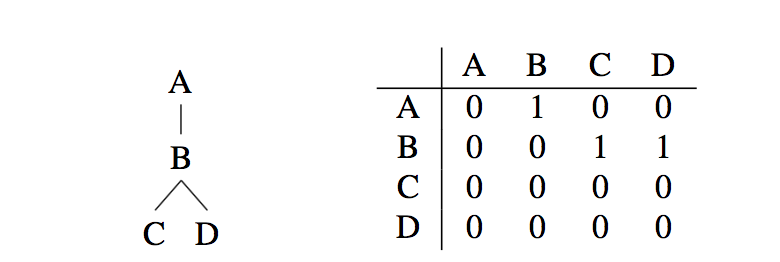
\includegraphics[width=6cm]{./figs/graph-matrix.png}
	\caption{4-graph example: Element of adjacency matrix is a binary string ``0100 0011 0000 0000", for which the decimal number is 17152}
	\label{fig:graph-ex}
	\end{figure}

	\item \textbf{Library Calls} \\ 
	If call of any contract from any other library occurs in the contract, addresses of all library contracts will be recorded. Similarity among them will be calculated with Jacobian similarity formula.
	%合约中如果发生调用其它库合约,所有库合约的地址也被记录下来,由雅克比相似度公式计算相似度。
	
	\item \textbf{Type Signature} \\
	This feature is composed of input parameter type and return parameter type, and similarity between them can be calculated with Jacobian similarity formula. For example, for the following smart contract code, feature of Type Signature of function ``getBalance" is vector (address, uint256). \\
	%该特征由输入参数类型和返回参数类型组成,由雅克比相似度公式计算相似度。例如对于下面的智能合约代码,函数getBalance的Type Signature特征为向量(address, uint256)。
	
	\begin{figure}[h]
  	\centering
  	\begin{minipage}{.7\linewidth}
	\begin{lstlisting}[frame=single]
contract addressTest {
  function getBalance(address addr) returns (uint) {
  	return addr.balance;
  }
}
	\end{lstlisting}
  	\end{minipage}
	\end{figure}

	\item \textbf{Local Types:} This feature is the set of all types of local variables of the function body, for which similarity should be calculated with Jacobian similarity formula.
	%该特征为函数体所有局部变量类型的集合,由雅克比相似度公式计算相似度。
	
	\item \textbf{Numeric Literals:} The set of all numeric constants serves as the feature of Numeric Literals, for which similarity should be calculated with Jacobian similarity formula.
	%所有数值常量的集合作为Numeric Literals特征,由雅克比相似度公式计算相似度。
	
	\item \textbf{String Literals:} The set of all string constants serves as the feature of String Literals, for which similarity should be calculated with Jacobian similarity formula.
	%所有字符串常量的集合作为String Literals特征,由雅克比相似度公式计算相似度。
\end{itemize}

Feature family can be expanded, so it is convenient to add new features to it. Based on the circumstance that there is a similarity calculation for each feature, we calculate the weighted sum of all features and thus can acquire the final code similarity:

%特征族可扩展,可以方便的把各种新的特征加入进来。基于每个特征都有一个相似度计算,我们把所有特征的相似度做加权和,得到最终的代码相似度:

\begin{equation}
	sim_{combined}(\vec{A}, \vec{B})=\frac{\sum_{c=1}^{n_{cl}}sim_{c}(\vec{A_c},~\vec{B_c})\cdot w_{c}}{\sum_{c=1}^{n_{cl}}w_{c}}
\end{equation}

Therein, $\vec{A}$ and $\vec{B}$ are eigenvectors; $n_{cl}$ is number of features in the feature family; $sim_{c}$ is similarity calculation function specific to feature c; $\vec{A_c}$ and $\vec{B_c}$ are eigenvectors of feature c; $w_{c}$ is weight of c. Weight can be acquired through machine learning algorithm training based on a large number of test sets.

%其中,$\vec{A}$和$\vec{B}$是特征向量;$n_{cl}$是特征族个数; $sim_{c}$是针对特征c的相似度计算函数;$\vec{A_c}$和$\vec{B_c}$是特征c的特征向量;$w_{c}$是特征c的权重。权重是可以在大量测试集上,通过机器学习算法训练得到的。
